\subsection{Product perspective}
\subsubsection{Class diagrams}
This section will present the high-level UML class diagrams of the application.
\\\\
\begin{figure}[H]
    \centering
    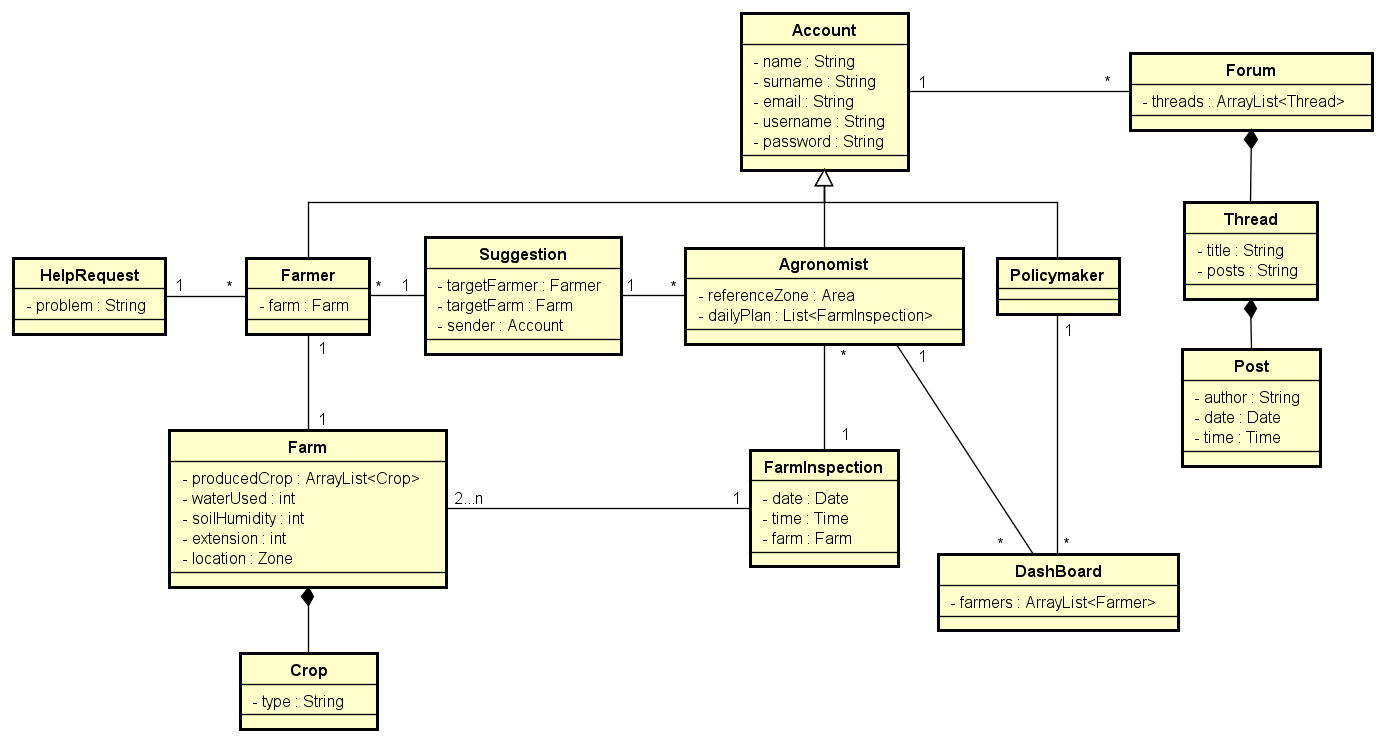
\includegraphics[width=\textwidth,height=\textheight,keepaspectratio]{Images/HighLevelUMLcut.png}
    \caption{\label{fig:high_level_uml}High level class diagram}
\end{figure}

\bigskip
\paragraph{Additional notes on the class diagram}
\begin{itemize}
    \item The agronomist attribute dailyPlan is a collection of FarmInspection ordered by date and time
    \item Both farmers and agronomists can create a suggestion responding to a farmer request
\end{itemize}

\newpage
\subsubsection{State machine diagrams}
The following diagrams are meant to give a high-level description of the states' evolution during the system processes.
\\\\

\begin{figure}[H]
    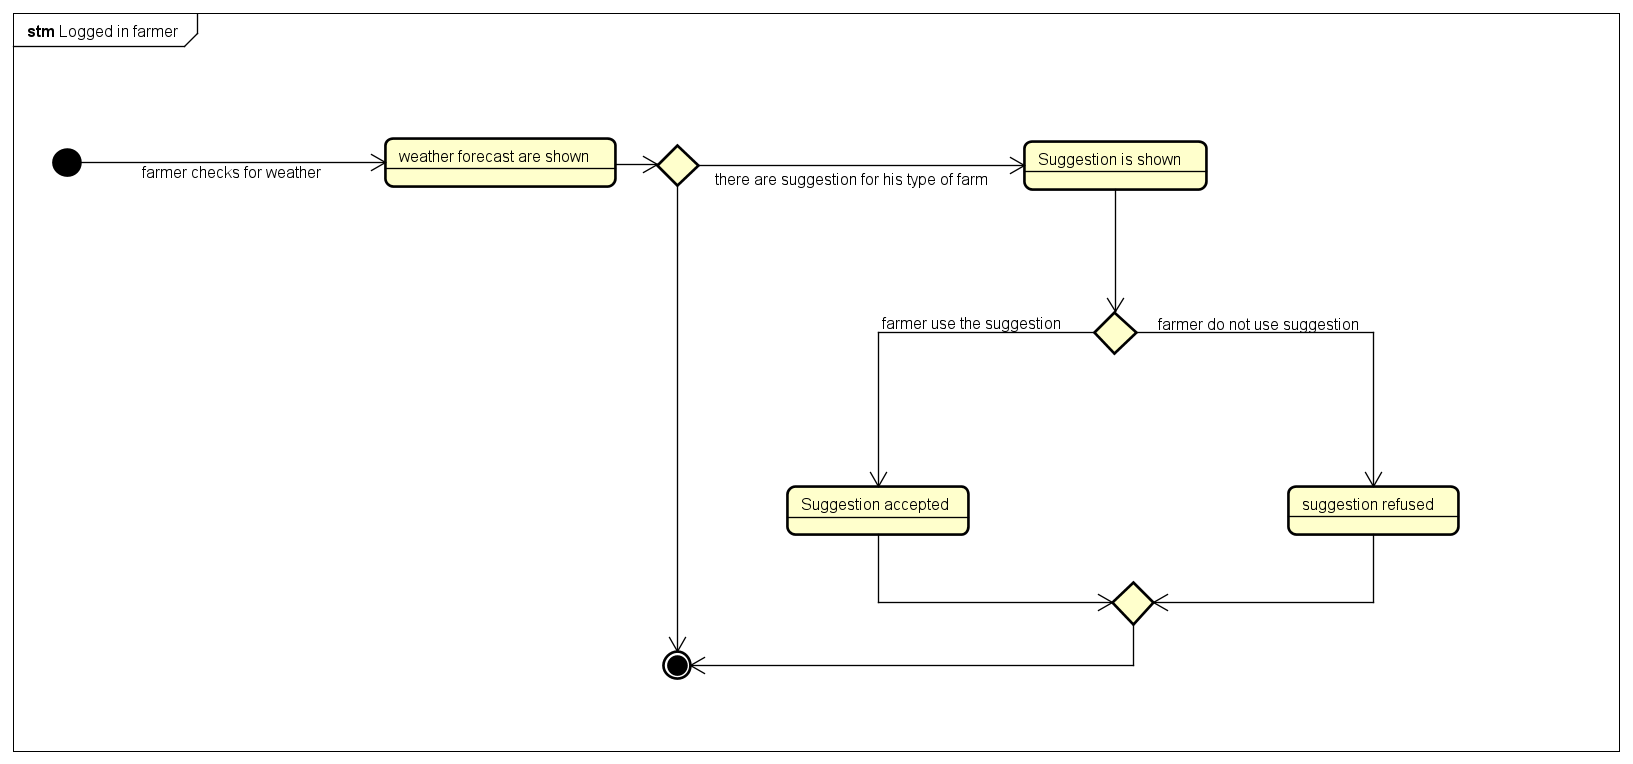
\includegraphics[width=\textwidth,height=\textheight,keepaspectratio]{Images/farmerChecksWeather.png}
    \caption{Statechart of a farmer checking weather forecast}
    \label{fig:statechart_farmer_weather}
\end{figure}

\begin{figure}[H]
    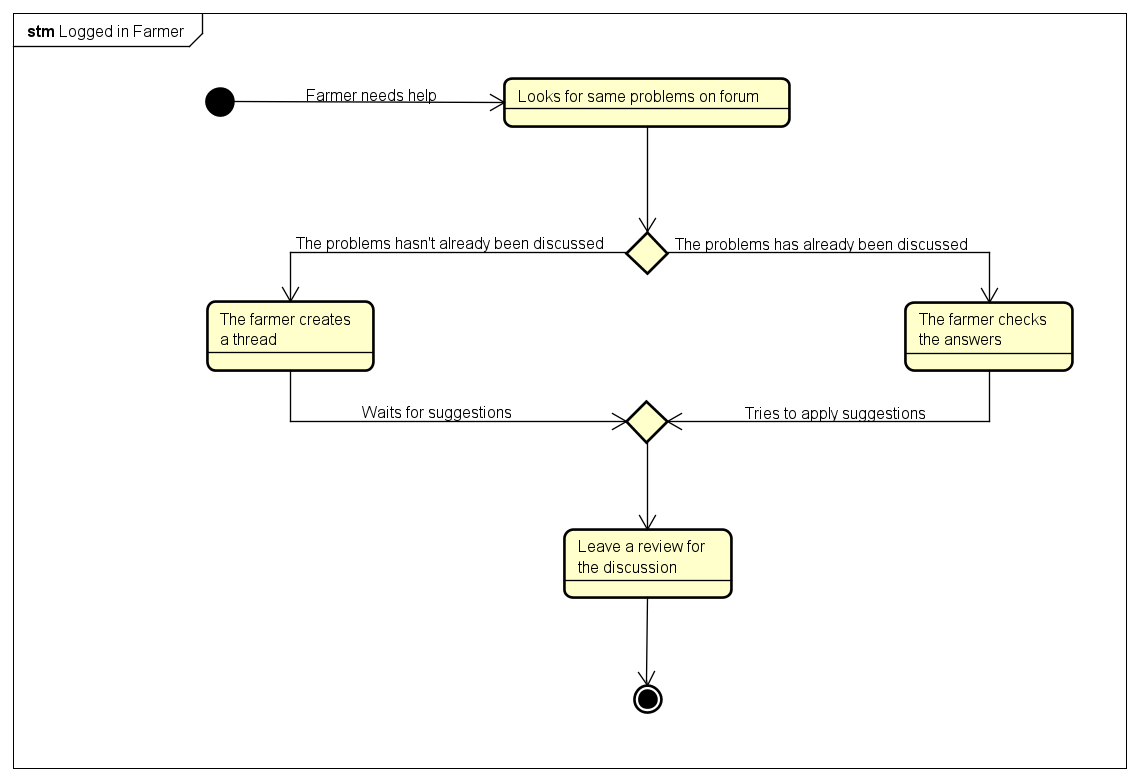
\includegraphics[width=\textwidth,height=\textheight,keepaspectratio]{Images/farmerCreatesThread.png}
    \caption{Statechart of the lifetime of a discussion thread on the forum}
    \label{fig:statechart_farmer_thread}
\end{figure}

\begin{figure}[H]
    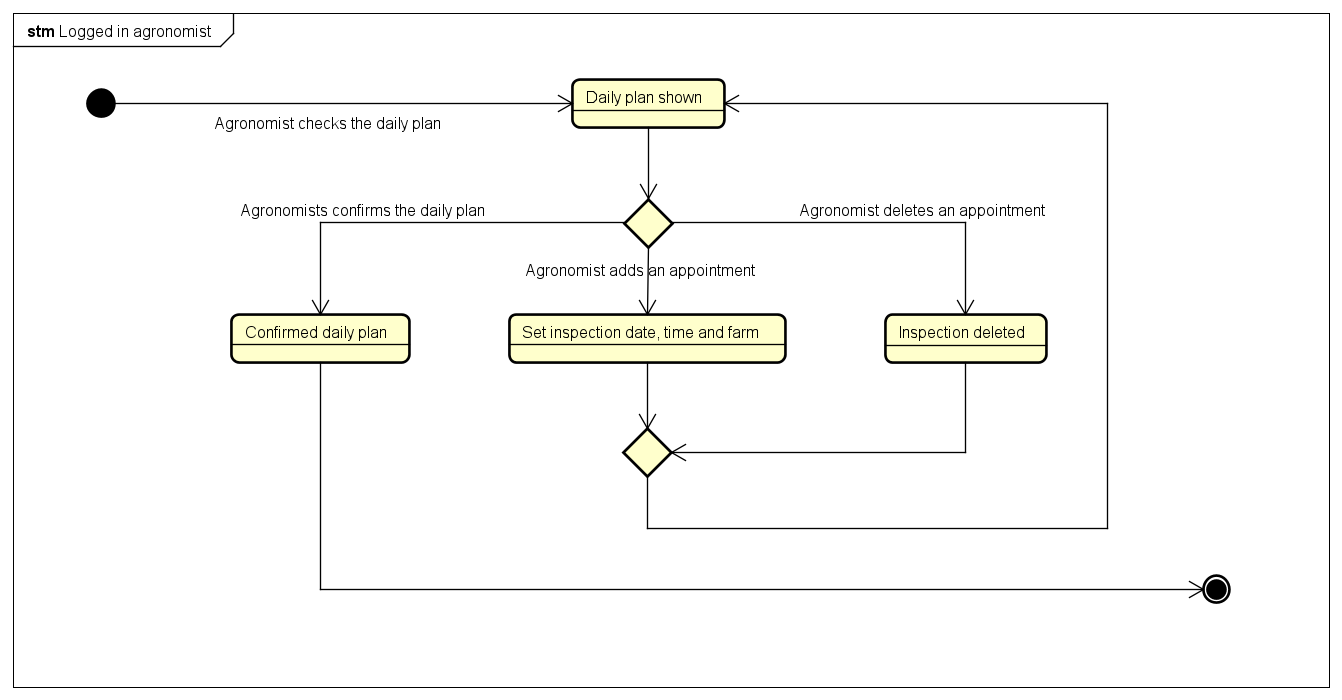
\includegraphics[width=\textwidth,height=\textheight,keepaspectratio]{Images/agronomistDailyPlan.png}
    \caption{Statechart of an agronomist managing his daily plan}
    \label{fig:statechart_agronomist_plan}
\end{figure}

\bigskip
\begin{figure}[H]
    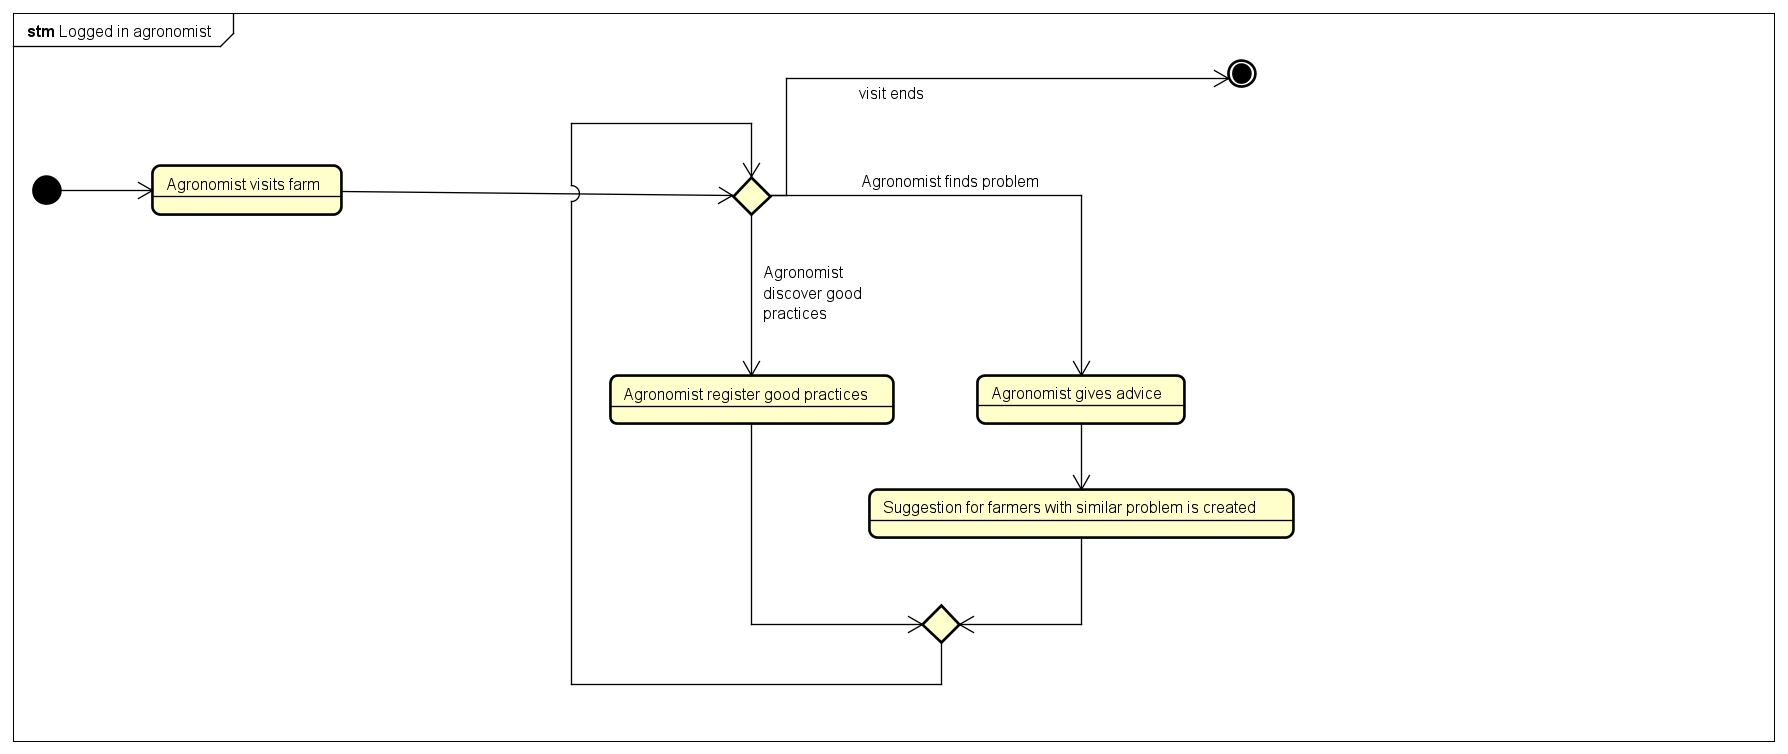
\includegraphics[width=\textwidth,height=\textheight,keepaspectratio]{Images/agronomistVisitFarm.png}
    \caption{Statechart of the lifetime of a farm visit}
    \label{fig:statechart_agronomist_visit}
\end{figure}
